\chapter{Results}

This chapter reports what the thirty-two completed runs produced. It follows the three research questions from the exposé: chart-reference agreement for RQ1; structural validity, completeness, and the unavailable human-rating layer for RQ2; and grounding plus perturbation robustness for RQ3. Model scale, model family, seed variability, failure modes, and computational cost are supporting analyses rather than separate research questions.

Every number in this chapter comes from a generated artifact. Run-level metrics come from the \texttt{metrics\_auto.json} file of each run; per-item outcomes, paired statistics and the three-level chart re-scoring come from \nolinkurl{experiments/results/final/dashboard_v4/statistics/}, produced by \nolinkurl{experiments/scripts/analyze_final_results.py}. Three reading rules apply throughout and are not repeated at every table. Chart agreement is agreement with the project's frozen reference recommendation and is an internal diagnostic, not independent evidence about visualization effectiveness. Seeds are repeated realisations of the same 274 held-out items and are shown individually rather than pooled. And every paired contrast carries the pair-level code-state label defined in Section 6.5.1; a significant result from a pair that is not code-state homogeneous shows that two runs differ, not that the method is the only reason they differ.

The chapter reports observations. Their interpretation, the failure analysis behind them, and the limits on what they license are the subject of Chapter 8.

\section{Structured-output reliability (RQ2: structure)}

Table 7.1 reports the structured-output quantities for every condition. The columns move from the weakest requirement to the strongest: whether a JSON object could be recovered at all, whether that object satisfied the runtime contract, whether every emitted mapping carried an object-valued encoding, and whether the raw object satisfied the strict response contract. Completeness is the mean fraction of the six required top-level fields that are present and non-empty.

The JSON-recovery column was recomputed from the stored raw text for all thirty-two runs so that runs written by different code vintages are comparable; the recomputed values match the \texttt{json\_parse\_rate} recorded in every one of the thirty-two \texttt{metrics\_auto.json} files exactly.

\begin{landscape}
\begingroup\scriptsize\setlength{\tabcolsep}{1pt}\sloppy
\begin{longtable}[]{@{}
  >{\raggedright\arraybackslash}p{(\linewidth - 14\tabcolsep) * \real{0.1000}}
  >{\raggedright\arraybackslash}p{(\linewidth - 14\tabcolsep) * \real{0.1000}}
  >{\raggedleft\arraybackslash}p{(\linewidth - 14\tabcolsep) * \real{0.1333}}
  >{\raggedleft\arraybackslash}p{(\linewidth - 14\tabcolsep) * \real{0.1333}}
  >{\raggedleft\arraybackslash}p{(\linewidth - 14\tabcolsep) * \real{0.1333}}
  >{\raggedleft\arraybackslash}p{(\linewidth - 14\tabcolsep) * \real{0.1333}}
  >{\raggedleft\arraybackslash}p{(\linewidth - 14\tabcolsep) * \real{0.1333}}
  >{\raggedleft\arraybackslash}p{(\linewidth - 14\tabcolsep) * \real{0.1333}}@{}}
\caption{Structured-output reliability, in percent unless stated otherwise. n = 274 held-out items per cell.}\tabularnewline
\toprule\noalign{}
\begin{minipage}[b]{\linewidth}\raggedright
Model
\end{minipage} & \begin{minipage}[b]{\linewidth}\raggedright
Method
\end{minipage} & \begin{minipage}[b]{\linewidth}\raggedleft
Seed
\end{minipage} & \begin{minipage}[b]{\linewidth}\raggedleft
JSON object recovered
\end{minipage} & \begin{minipage}[b]{\linewidth}\raggedleft
Runtime contract satisfied
\end{minipage} & \begin{minipage}[b]{\linewidth}\raggedleft
Encoding object valid
\end{minipage} & \begin{minipage}[b]{\linewidth}\raggedleft
Strict schema valid
\end{minipage} & \begin{minipage}[b]{\linewidth}\raggedleft
Completeness (0--1)
\end{minipage} \\
\midrule\noalign{}
\endfirsthead
\toprule\noalign{}
\begin{minipage}[b]{\linewidth}\raggedright
Model
\end{minipage} & \begin{minipage}[b]{\linewidth}\raggedright
Method
\end{minipage} & \begin{minipage}[b]{\linewidth}\raggedleft
Seed
\end{minipage} & \begin{minipage}[b]{\linewidth}\raggedleft
JSON object recovered
\end{minipage} & \begin{minipage}[b]{\linewidth}\raggedleft
Runtime contract satisfied
\end{minipage} & \begin{minipage}[b]{\linewidth}\raggedleft
Encoding object valid
\end{minipage} & \begin{minipage}[b]{\linewidth}\raggedleft
Strict schema valid
\end{minipage} & \begin{minipage}[b]{\linewidth}\raggedleft
Completeness (0--1)
\end{minipage} \\
\midrule\noalign{}
\endhead
\bottomrule\noalign{}
\endlastfoot
Qwen3-1.7B & A & 42 & 99.64 & 0.36 & 0.36 & 0.36 & 0.996 \\
Qwen3-1.7B & A & 43 & 100.00 & 0.00 & 0.00 & 0.00 & 1.000 \\
Qwen3-1.7B & A & 44 & 100.00 & 0.36 & 0.36 & 0.36 & 1.000 \\
Qwen3-1.7B & B & 42 & 100.00 & 1.09 & 1.09 & 1.09 & 1.000 \\
Qwen3-1.7B & B & 43 & 99.64 & 1.46 & 1.46 & 1.46 & 0.996 \\
Qwen3-1.7B & B & 44 & 100.00 & 1.09 & 1.09 & 1.09 & 1.000 \\
Qwen3-1.7B & C & 42 & 97.45 & 1.46 & 1.46 & 1.46 & 0.974 \\
Qwen3-1.7B & C & 43 & 83.94 & 83.94 & 83.94 & 0.00 & 0.839 \\
Qwen3-1.7B & C & 44 & 87.96 & 87.96 & 87.96 & 0.00 & 0.880 \\
Qwen3-1.7B & D & 42 & 95.99 & 0.00 & 0.00 & 0.00 & 0.958 \\
Qwen3-1.7B & D & 43 & 98.54 & 98.54 & 98.54 & 0.00 & 0.985 \\
Qwen3-1.7B & D & 44 & 100.00 & 100.00 & 100.00 & 0.00 & 1.000 \\
Qwen3-8B & A & 42 & 100.00 & 100.00 & 100.00 & 0.00 & 1.000 \\
Qwen3-8B & B & 42 & 100.00 & 100.00 & 100.00 & 0.00 & 1.000 \\
Qwen3-8B & C & 42 & 86.13 & 86.13 & 86.13 & 0.00 & 0.861 \\
Qwen3-8B & D & 42 & 74.09 & 74.09 & 74.09 & 0.00 & 0.741 \\
Qwen3.8-27B & A & 42 & 100.00 & 100.00 & 100.00 & 46.72 & 1.000 \\
Qwen3.8-27B & B & 42 & 100.00 & 100.00 & 100.00 & 84.67 & 0.999 \\
Qwen3.8-27B & C & 42 & 100.00 & 100.00 & 100.00 & 0.00 & 1.000 \\
Qwen3.8-27B & D & 42 & 100.00 & 100.00 & 100.00 & 0.00 & 1.000 \\
OLMo-2-1B-Instruct & A & 42 & 30.29 & 26.28 & 12.04 & 0.00 & 0.248 \\
OLMo-2-1B-Instruct & A & 43 & 32.85 & 27.74 & 10.22 & 0.00 & 0.265 \\
OLMo-2-1B-Instruct & A & 44 & 32.12 & 27.01 & 12.04 & 0.00 & 0.257 \\
OLMo-2-1B-Instruct & B & 42 & 46.35 & 38.32 & 9.85 & 0.00 & 0.368 \\
OLMo-2-1B-Instruct & B & 43 & 49.64 & 42.70 & 9.85 & 0.00 & 0.391 \\
OLMo-2-1B-Instruct & B & 44 & 47.08 & 38.69 & 9.12 & 0.00 & 0.381 \\
OLMo-2-1B-Instruct & C & 42 & 2.92 & 2.92 & 2.92 & 0.00 & 0.029 \\
OLMo-2-1B-Instruct & C & 43 & 2.92 & 2.92 & 2.92 & 0.00 & 0.029 \\
OLMo-2-1B-Instruct & C & 44 & 2.92 & 2.92 & 2.92 & 0.00 & 0.029 \\
OLMo-2-1B-Instruct & D & 42 & 1.09 & 1.09 & 1.09 & 0.00 & 0.011 \\
OLMo-2-1B-Instruct & D & 43 & 2.55 & 2.55 & 2.55 & 0.00 & 0.026 \\
OLMo-2-1B-Instruct & D & 44 & 3.28 & 3.28 & 3.28 & 0.00 & 0.033 \\
\end{longtable}
\endgroup
\end{landscape}

Five observations follow directly from Table 7.1.

\textbf{The two largest models satisfy the output contract without adaptation.} Qwen3-8B and Qwen3.8-27B both recover a JSON object and satisfy the runtime contract on 274 of 274 items in the prompt-only and RAG conditions. Neither needs fine-tuning to produce a machine-readable record.

\textbf{Fine-tuning does not preserve that property at 8B.} Qwen3-8B falls from 100 \% contract satisfaction under A and B to 86.13 \% under C and 74.09 \% under D. The drop is significant on the paired test (C \ensuremath{-} A = \ensuremath{-}13.87 pp, Holm-adjusted p = 2.9 \(\times\) \(10^{-11}\); D \ensuremath{-} C = \ensuremath{-}12.04 pp, p = 2.1 \(\times\) \(10^{-8}\), and this second contrast comes from a code-state homogeneous pair). Section 7.5 shows that the lost items are truncated, not malformed.

\textbf{Recovering a JSON object and satisfying the contract are very different things at 1.7B.} In the prompt-only and RAG conditions, Qwen3-1.7B produces a recoverable JSON object on essentially every item (99.6--100 \%) but satisfies the runtime contract on at most 1.5 \%. The gap is a single recurring type error: the model emits \texttt{encoding} as a string --- the name of one column --- where the contract requires an object with named channels. The same failure appears in the seed-42 fine-tuned runs, which were produced by an earlier code and training state; the seed-43 and seed-44 adapters trained under the current state removed it, raising contract satisfaction from 1.5 \% to 84--99 \%.

\textbf{Strict schema validity behaves inversely to reference fidelity, as predicted in Section 6.6.3.} Every fine-tuned condition scores 0.00 \%, as do both Qwen3-8B base-model conditions, while the two 27B base-model conditions score 46.72 \% and 84.67 \%. This is not a quality ordering. The strict contract forbids extra keys in the encoding object, and the frozen reference encodings carry thirteen additional source-grounded keys. Applying the strict contract to the 274 reference recommendations themselves yields \textbf{0 of 274 passing}, with the violations concentrated entirely on those extra keys. A model that has learned to reproduce the reference format therefore \emph{must} score 0 \%, and a model that emits a minimal encoding scores well. Strict schema validity is reported here for completeness and is excluded from every comparative statement in this thesis.

\textbf{Retrieval helps output recoverability only where it is missing.} For OLMo, retrieval raises JSON recovery by 15--17 pp across all three seeds. For Qwen3-8B and Qwen3.8-27B, where recovery is already complete, it changes nothing: every B \ensuremath{-} A contrast on that outcome has zero discordant items.

Table 7.2 gives the paired tests for JSON recovery in the blocks where a difference exists.

\begin{landscape}
\begingroup\scriptsize\setlength{\tabcolsep}{1pt}\sloppy
\begin{longtable}[]{@{}
  >{\raggedright\arraybackslash}p{(\linewidth - 14\tabcolsep) * \real{0.1071}}
  >{\raggedleft\arraybackslash}p{(\linewidth - 14\tabcolsep) * \real{0.1429}}
  >{\raggedright\arraybackslash}p{(\linewidth - 14\tabcolsep) * \real{0.1071}}
  >{\raggedleft\arraybackslash}p{(\linewidth - 14\tabcolsep) * \real{0.1429}}
  >{\raggedright\arraybackslash}p{(\linewidth - 14\tabcolsep) * \real{0.1071}}
  >{\raggedleft\arraybackslash}p{(\linewidth - 14\tabcolsep) * \real{0.1429}}
  >{\raggedleft\arraybackslash}p{(\linewidth - 14\tabcolsep) * \real{0.1429}}
  >{\raggedright\arraybackslash}p{(\linewidth - 14\tabcolsep) * \real{0.1071}}@{}}
\caption{Paired contrasts on JSON recovery, restricted to contrasts with at least one discordant item. Difference in percentage points with a 95 \% bootstrap interval; \emph{p} is the Holm-corrected exact McNemar value within the block; b+c is the number of discordant items; the last column is the code state of the two runs being contrasted.}\tabularnewline
\toprule\noalign{}
\begin{minipage}[b]{\linewidth}\raggedright
Model
\end{minipage} & \begin{minipage}[b]{\linewidth}\raggedleft
Seed
\end{minipage} & \begin{minipage}[b]{\linewidth}\raggedright
Contrast
\end{minipage} & \begin{minipage}[b]{\linewidth}\raggedleft
\(\Delta\) (pp)
\end{minipage} & \begin{minipage}[b]{\linewidth}\raggedright
95 \% CI
\end{minipage} & \begin{minipage}[b]{\linewidth}\raggedleft
b+c
\end{minipage} & \begin{minipage}[b]{\linewidth}\raggedleft
\emph{p} (Holm)
\end{minipage} & \begin{minipage}[b]{\linewidth}\raggedright
Pair code state
\end{minipage} \\
\midrule\noalign{}
\endfirsthead
\toprule\noalign{}
\begin{minipage}[b]{\linewidth}\raggedright
Model
\end{minipage} & \begin{minipage}[b]{\linewidth}\raggedleft
Seed
\end{minipage} & \begin{minipage}[b]{\linewidth}\raggedright
Contrast
\end{minipage} & \begin{minipage}[b]{\linewidth}\raggedleft
\(\Delta\) (pp)
\end{minipage} & \begin{minipage}[b]{\linewidth}\raggedright
95 \% CI
\end{minipage} & \begin{minipage}[b]{\linewidth}\raggedleft
b+c
\end{minipage} & \begin{minipage}[b]{\linewidth}\raggedleft
\emph{p} (Holm)
\end{minipage} & \begin{minipage}[b]{\linewidth}\raggedright
Pair code state
\end{minipage} \\
\midrule\noalign{}
\endhead
\bottomrule\noalign{}
\endlastfoot
OLMo-2-1B & 42 & B \ensuremath{-} A & +16.06 & {[}+7.66, +24.45{]} & 148 & 7.5 \(\times\) \(10^{-4}\) & homogeneous \\
OLMo-2-1B & 43 & B \ensuremath{-} A & +16.79 & {[}+8.76, +24.82{]} & 128 & 1.2 \(\times\) \(10^{-4}\) & unknown \\
OLMo-2-1B & 44 & B \ensuremath{-} A & +14.96 & {[}+6.57, +22.99{]} & 135 & 1.1 \(\times\) \(10^{-3}\) & unknown \\
OLMo-2-1B & 42 & C \ensuremath{-} A & \ensuremath{-}27.37 & {[}\ensuremath{-}33.21, \ensuremath{-}21.53{]} & 87 & 2.1 \(\times\) \(10^{-17}\) & mixed \\
OLMo-2-1B & 43 & C \ensuremath{-} A & \ensuremath{-}29.93 & {[}\ensuremath{-}35.77, \ensuremath{-}24.09{]} & 90 & 1.3 \(\times\) \(10^{-20}\) & unknown \\
OLMo-2-1B & 44 & C \ensuremath{-} A & \ensuremath{-}29.20 & {[}\ensuremath{-}35.04, \ensuremath{-}23.36{]} & 90 & 3.0 \(\times\) \(10^{-19}\) & unknown \\
Qwen3-1.7B & 43 & C \ensuremath{-} A & \ensuremath{-}16.06 & {[}\ensuremath{-}20.44, \ensuremath{-}11.68{]} & 44 & 6.8 \(\times\) \(10^{-13}\) & unknown \\
Qwen3-1.7B & 44 & C \ensuremath{-} A & \ensuremath{-}12.04 & {[}\ensuremath{-}16.06, \ensuremath{-}8.39{]} & 33 & 1.4 \(\times\) \(10^{-9}\) & unknown \\
Qwen3-1.7B & 43 & D \ensuremath{-} C & +14.60 & {[}+10.22, +18.98{]} & 44 & 4.5 \(\times\) \(10^{-10}\) & mixed \\
Qwen3-1.7B & 44 & D \ensuremath{-} C & +12.04 & {[}+8.39, +16.06{]} & 33 & 1.4 \(\times\) \(10^{-9}\) & mixed \\
Qwen3-8B & 42 & C \ensuremath{-} A & \ensuremath{-}13.87 & {[}\ensuremath{-}18.25, \ensuremath{-}9.85{]} & 38 & 2.9 \(\times\) \(10^{-11}\) & mixed \\
Qwen3-8B & 42 & D \ensuremath{-} C & \ensuremath{-}12.04 & {[}\ensuremath{-}16.42, \ensuremath{-}8.03{]} & 37 & 2.1 \(\times\) \(10^{-8}\) & homogeneous \\
Qwen3-8B & 42 & D \ensuremath{-} B & \ensuremath{-}25.91 & {[}\ensuremath{-}31.02, \ensuremath{-}20.80{]} & 71 & 5.1 \(\times\) \(10^{-21}\) & mixed \\
\end{longtable}
\endgroup
\end{landscape}

Adding fine-tuning lowers JSON recovery in every model where it has room to fall: by 27--30 pp for OLMo, by 12--16 pp for Qwen3-1.7B seeds 43 and 44, and by 13.87 pp for Qwen3-8B. At 27B nothing changes, because every condition already succeeds on every item.

\section{Chart agreement at three levels of strictness (RQ1)}

\begin{figure}[tbp]
  \centering
  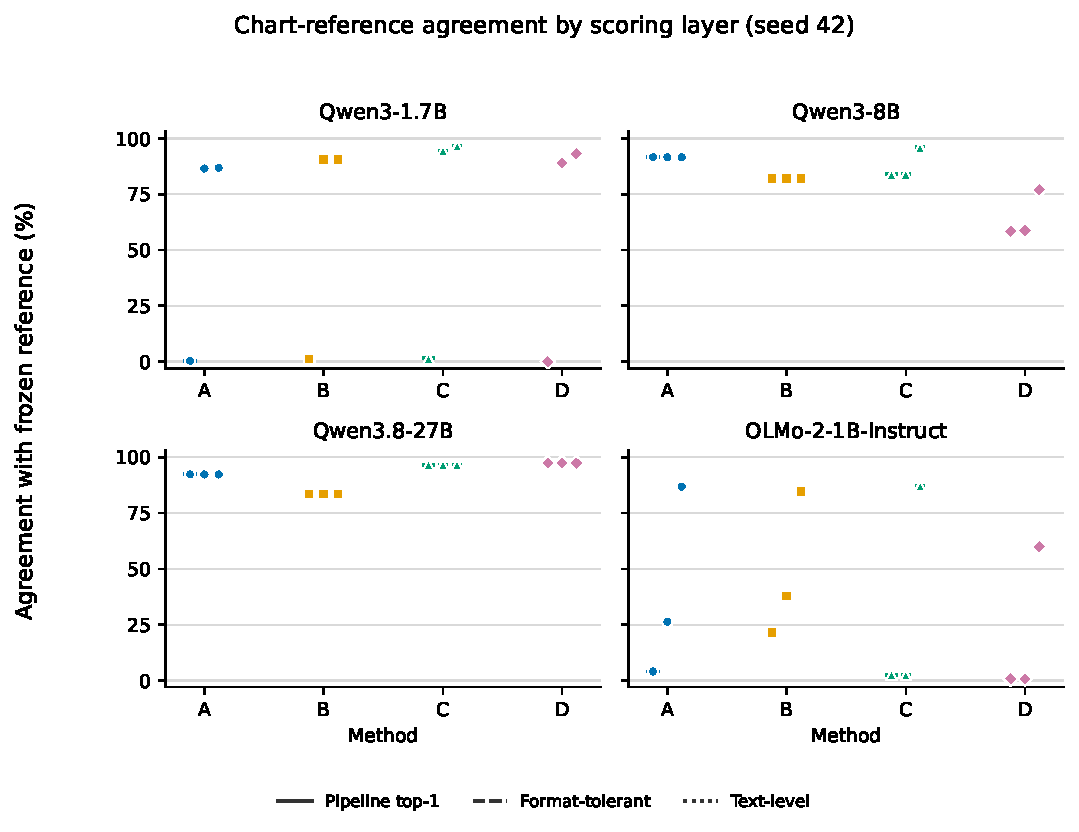
\includegraphics[width=\textwidth]{figures/chart_agreement_decomposition.pdf}
  \caption{Agreement with the frozen chart reference at three scoring layers for seed 42. The layers separate end-to-end pipeline success from format-tolerant and text-level recovery. Values are internal reference-agreement diagnostics, not independent evidence of visualization effectiveness. Methods are A (prompt-only), B (RAG), C (QLoRA), and D (QLoRA+RAG). Source: \texttt{tables/format\_tolerant\_chart\_accuracy.csv}.}
  \label{fig:chart-agreement-decomposition}
\end{figure}


Section 6.6.5 defined three levels at which the primary chart decision can be compared with the reference. Table 7.3 reports all three side by side, together with the number of responses whose outermost JSON object was never closed.

\begin{landscape}
\begingroup\scriptsize\setlength{\tabcolsep}{1pt}\sloppy
\begin{longtable}[]{@{}
  >{\raggedright\arraybackslash}p{(\linewidth - 14\tabcolsep) * \real{0.1000}}
  >{\raggedright\arraybackslash}p{(\linewidth - 14\tabcolsep) * \real{0.1000}}
  >{\raggedleft\arraybackslash}p{(\linewidth - 14\tabcolsep) * \real{0.1333}}
  >{\raggedleft\arraybackslash}p{(\linewidth - 14\tabcolsep) * \real{0.1333}}
  >{\raggedleft\arraybackslash}p{(\linewidth - 14\tabcolsep) * \real{0.1333}}
  >{\raggedleft\arraybackslash}p{(\linewidth - 14\tabcolsep) * \real{0.1333}}
  >{\raggedleft\arraybackslash}p{(\linewidth - 14\tabcolsep) * \real{0.1333}}
  >{\raggedleft\arraybackslash}p{(\linewidth - 14\tabcolsep) * \real{0.1333}}@{}}
\caption{Primary-chart agreement in percent at three levels of strictness, and truncated responses out of 274. Levels 2 and 3 are post-hoc diagnostics computed from the stored raw text; level 1 is the pre-specified metric.}\tabularnewline
\toprule\noalign{}
\begin{minipage}[b]{\linewidth}\raggedright
Model
\end{minipage} & \begin{minipage}[b]{\linewidth}\raggedright
Method
\end{minipage} & \begin{minipage}[b]{\linewidth}\raggedleft
Seed
\end{minipage} & \begin{minipage}[b]{\linewidth}\raggedleft
Truncated
\end{minipage} & \begin{minipage}[b]{\linewidth}\raggedleft
(1) Pipeline top-1
\end{minipage} & \begin{minipage}[b]{\linewidth}\raggedleft
(2) Format-tolerant
\end{minipage} & \begin{minipage}[b]{\linewidth}\raggedleft
(3) Text-level
\end{minipage} & \begin{minipage}[b]{\linewidth}\raggedleft
(3) \ensuremath{-} (1)
\end{minipage} \\
\midrule\noalign{}
\endfirsthead
\toprule\noalign{}
\begin{minipage}[b]{\linewidth}\raggedright
Model
\end{minipage} & \begin{minipage}[b]{\linewidth}\raggedright
Method
\end{minipage} & \begin{minipage}[b]{\linewidth}\raggedleft
Seed
\end{minipage} & \begin{minipage}[b]{\linewidth}\raggedleft
Truncated
\end{minipage} & \begin{minipage}[b]{\linewidth}\raggedleft
(1) Pipeline top-1
\end{minipage} & \begin{minipage}[b]{\linewidth}\raggedleft
(2) Format-tolerant
\end{minipage} & \begin{minipage}[b]{\linewidth}\raggedleft
(3) Text-level
\end{minipage} & \begin{minipage}[b]{\linewidth}\raggedleft
(3) \ensuremath{-} (1)
\end{minipage} \\
\midrule\noalign{}
\endhead
\bottomrule\noalign{}
\endlastfoot
Qwen3-1.7B & A & 42 & 0 & 0.36 & 86.50 & 86.86 & +86.50 \\
Qwen3-1.7B & A & 43 & 0 & 0.00 & 87.23 & 87.23 & +87.23 \\
Qwen3-1.7B & A & 44 & 0 & 0.36 & 86.86 & 86.86 & +86.50 \\
Qwen3-1.7B & B & 42 & 0 & 1.09 & 90.51 & 90.51 & +89.42 \\
Qwen3-1.7B & B & 43 & 0 & 1.09 & 89.78 & 90.15 & +89.06 \\
Qwen3-1.7B & B & 44 & 0 & 1.09 & 89.05 & 89.05 & +87.96 \\
Qwen3-1.7B & C & 42 & 1 & 1.46 & 94.53 & 96.72 & +95.26 \\
Qwen3-1.7B & C & 43 & 38 & 80.66 & 81.02 & 96.72 & +16.06 \\
Qwen3-1.7B & C & 44 & 29 & 85.40 & 85.40 & 97.45 & +12.05 \\
Qwen3-1.7B & D & 42 & 1 & 0.00 & 89.05 & 93.07 & +93.07 \\
Qwen3-1.7B & D & 43 & 0 & 89.42 & 89.42 & 90.88 & +1.46 \\
Qwen3-1.7B & D & 44 & 0 & 89.05 & 89.05 & 89.05 & 0.00 \\
Qwen3-8B & A & 42 & 0 & 91.61 & 91.61 & 91.61 & 0.00 \\
Qwen3-8B & B & 42 & 0 & 82.12 & 82.12 & 82.12 & 0.00 \\
Qwen3-8B & C & 42 & 36 & 83.94 & 83.94 & 95.99 & +12.05 \\
Qwen3-8B & D & 42 & 69 & 58.39 & 58.76 & 77.01 & +18.62 \\
Qwen3.8-27B & A & 42 & 0 & 92.34 & 92.34 & 92.34 & 0.00 \\
Qwen3.8-27B & B & 42 & 0 & 83.58 & 83.58 & 83.58 & 0.00 \\
Qwen3.8-27B & C & 42 & 0 & 96.72 & 96.72 & 96.72 & 0.00 \\
Qwen3.8-27B & D & 42 & 0 & 97.45 & 97.45 & 97.45 & 0.00 \\
OLMo-2-1B & A & 42 & 272 & 4.01 & 26.28 & 86.86 & +82.85 \\
OLMo-2-1B & A & 43 & 272 & 6.93 & 28.83 & 87.59 & +80.66 \\
OLMo-2-1B & A & 44 & 273 & 5.11 & 30.29 & 86.13 & +81.02 \\
OLMo-2-1B & B & 42 & 274 & 21.53 & 37.96 & 84.67 & +63.14 \\
OLMo-2-1B & B & 43 & 274 & 24.09 & 41.61 & 83.58 & +59.49 \\
OLMo-2-1B & B & 44 & 272 & 23.36 & 40.51 & 85.77 & +62.41 \\
OLMo-2-1B & C & 42 & 256 & 2.55 & 2.55 & 87.23 & +84.68 \\
OLMo-2-1B & C & 43 & 254 & 2.92 & 2.92 & 93.43 & +90.51 \\
OLMo-2-1B & C & 44 & 258 & 2.92 & 2.92 & 94.89 & +91.97 \\
OLMo-2-1B & D & 42 & 264 & 0.73 & 0.73 & 59.85 & +59.12 \\
OLMo-2-1B & D & 43 & 262 & 2.19 & 2.19 & 56.93 & +54.74 \\
OLMo-2-1B & D & 44 & 258 & 2.92 & 2.92 & 66.06 & +63.14 \\
\end{longtable}
\endgroup
\end{landscape}

The final column is the central result of this chapter. It is zero for every 27B condition and for the two Qwen3-8B base-model conditions: there the pipeline metric and the raw text agree completely, because every response is a complete, contract-valid object. Everywhere else it is large, and it is large for two distinct reasons that the three levels separate.

For Qwen3-1.7B in conditions A and B, the responses are complete and decodable --- zero truncations --- but fail the runtime contract because of the string-valued \texttt{encoding} field. Level 2 already recovers the chart decision: 86.5--90.5 \% agreement against a pipeline value below 1.5 \%. Here the gap is entirely the cost of the runtime contract.

For OLMo in every condition, and for the fine-tuned Qwen3-8B and Qwen3-1.7B conditions with non-zero truncation counts, the second gap appears. OLMo truncates on 254--274 of 274 items in every condition: the model produces a well-formed and often correct prefix and then runs out of the 512-token budget before the outermost object can be closed. Level 3 recovers 84--95 \% chart agreement from those prefixes in the A, B and C conditions.

Table 7.4 gives the omnibus test across the four methods for the two chart levels.

\begin{landscape}
\begingroup\scriptsize\setlength{\tabcolsep}{1pt}\sloppy
\begin{longtable}[]{@{}
  >{\raggedright\arraybackslash}p{(\linewidth - 16\tabcolsep) * \real{0.0882}}
  >{\raggedleft\arraybackslash}p{(\linewidth - 16\tabcolsep) * \real{0.1176}}
  >{\raggedright\arraybackslash}p{(\linewidth - 16\tabcolsep) * \real{0.0882}}
  >{\raggedleft\arraybackslash}p{(\linewidth - 16\tabcolsep) * \real{0.1176}}
  >{\raggedleft\arraybackslash}p{(\linewidth - 16\tabcolsep) * \real{0.1176}}
  >{\raggedleft\arraybackslash}p{(\linewidth - 16\tabcolsep) * \real{0.1176}}
  >{\raggedleft\arraybackslash}p{(\linewidth - 16\tabcolsep) * \real{0.1176}}
  >{\raggedleft\arraybackslash}p{(\linewidth - 16\tabcolsep) * \real{0.1176}}
  >{\raggedleft\arraybackslash}p{(\linewidth - 16\tabcolsep) * \real{0.1176}}@{}}
\caption{Cochran's Q across methods A--D on matched items (n = 274, df = 3). Rates are per-condition agreement in percent.}\tabularnewline
\toprule\noalign{}
\begin{minipage}[b]{\linewidth}\raggedright
Model
\end{minipage} & \begin{minipage}[b]{\linewidth}\raggedleft
Seed
\end{minipage} & \begin{minipage}[b]{\linewidth}\raggedright
Outcome
\end{minipage} & \begin{minipage}[b]{\linewidth}\raggedleft
A
\end{minipage} & \begin{minipage}[b]{\linewidth}\raggedleft
B
\end{minipage} & \begin{minipage}[b]{\linewidth}\raggedleft
C
\end{minipage} & \begin{minipage}[b]{\linewidth}\raggedleft
D
\end{minipage} & \begin{minipage}[b]{\linewidth}\raggedleft
Q
\end{minipage} & \begin{minipage}[b]{\linewidth}\raggedleft
\emph{p}
\end{minipage} \\
\midrule\noalign{}
\endfirsthead
\toprule\noalign{}
\begin{minipage}[b]{\linewidth}\raggedright
Model
\end{minipage} & \begin{minipage}[b]{\linewidth}\raggedleft
Seed
\end{minipage} & \begin{minipage}[b]{\linewidth}\raggedright
Outcome
\end{minipage} & \begin{minipage}[b]{\linewidth}\raggedleft
A
\end{minipage} & \begin{minipage}[b]{\linewidth}\raggedleft
B
\end{minipage} & \begin{minipage}[b]{\linewidth}\raggedleft
C
\end{minipage} & \begin{minipage}[b]{\linewidth}\raggedleft
D
\end{minipage} & \begin{minipage}[b]{\linewidth}\raggedleft
Q
\end{minipage} & \begin{minipage}[b]{\linewidth}\raggedleft
\emph{p}
\end{minipage} \\
\midrule\noalign{}
\endhead
\bottomrule\noalign{}
\endlastfoot
Qwen3-1.7B & 42 & pipeline top-1 & 0.36 & 1.09 & 1.46 & 0.00 & 5.00 & 0.172 \\
Qwen3-1.7B & 43 & pipeline top-1 & 0.00 & 1.09 & 80.66 & 89.42 & 657.80 & 3.0 \(\times\) \(10^{-142}\) \\
Qwen3-1.7B & 44 & pipeline top-1 & 0.36 & 1.09 & 85.40 & 89.05 & 671.96 & 2.5 \(\times\) \(10^{-145}\) \\
Qwen3-1.7B & 42 & text-level & 86.86 & 90.51 & 96.72 & 93.07 & 34.84 & 1.3 \(\times\) \(10^{-7}\) \\
Qwen3-1.7B & 43 & text-level & 87.23 & 90.15 & 96.72 & 90.88 & 28.86 & 2.4 \(\times\) \(10^{-6}\) \\
Qwen3-1.7B & 44 & text-level & 86.86 & 89.05 & 97.45 & 89.05 & 33.79 & 2.2 \(\times\) \(10^{-7}\) \\
Qwen3-8B & 42 & pipeline top-1 & 91.61 & 82.12 & 83.94 & 58.39 & 133.12 & 1.2 \(\times\) \(10^{-28}\) \\
Qwen3-8B & 42 & text-level & 91.61 & 82.12 & 95.99 & 77.01 & 75.16 & 3.4 \(\times\) \(10^{-16}\) \\
Qwen3.8-27B & 42 & pipeline top-1 & 92.34 & 83.58 & 96.72 & 97.45 & 84.46 & 3.4 \(\times\) \(10^{-18}\) \\
Qwen3.8-27B & 42 & text-level & 92.34 & 83.58 & 96.72 & 97.45 & 84.46 & 3.4 \(\times\) \(10^{-18}\) \\
OLMo-2-1B & 42 & pipeline top-1 & 4.01 & 21.53 & 2.55 & 0.73 & 111.72 & 4.7 \(\times\) \(10^{-24}\) \\
OLMo-2-1B & 43 & pipeline top-1 & 6.93 & 24.09 & 2.92 & 2.19 & 110.51 & 8.5 \(\times\) \(10^{-24}\) \\
OLMo-2-1B & 44 & pipeline top-1 & 5.11 & 23.36 & 2.92 & 2.92 & 104.46 & 1.7 \(\times\) \(10^{-22}\) \\
OLMo-2-1B & 42 & text-level & 86.86 & 84.67 & 87.23 & 59.85 & 110.05 & 1.1 \(\times\) \(10^{-23}\) \\
OLMo-2-1B & 43 & text-level & 87.59 & 83.58 & 93.43 & 56.93 & 158.37 & 4.1 \(\times\) \(10^{-34}\) \\
OLMo-2-1B & 44 & text-level & 86.13 & 85.77 & 94.89 & 66.06 & 114.72 & 1.1 \(\times\) \(10^{-24}\) \\
\end{longtable}
\endgroup
\end{landscape}

The omnibus test rejects the hypothesis of equal method performance in every block except Qwen3-1.7B seed 42 on the pipeline metric, where all four conditions fail almost every item and there is nothing to distinguish.

\subsection{The pipeline contrasts}

Table 7.5 reports the four planned contrasts on the pre-specified metric.

\begin{landscape}
\begingroup\scriptsize\setlength{\tabcolsep}{3pt}\sloppy
\begin{longtable}[]{@{}
  >{\raggedright\arraybackslash}p{(\linewidth - 10\tabcolsep) * \real{0.1579}}
  >{\raggedleft\arraybackslash}p{(\linewidth - 10\tabcolsep) * \real{0.2105}}
  >{\raggedright\arraybackslash}p{(\linewidth - 10\tabcolsep) * \real{0.1579}}
  >{\raggedright\arraybackslash}p{(\linewidth - 10\tabcolsep) * \real{0.1579}}
  >{\raggedright\arraybackslash}p{(\linewidth - 10\tabcolsep) * \real{0.1579}}
  >{\raggedright\arraybackslash}p{(\linewidth - 10\tabcolsep) * \real{0.1579}}@{}}
\caption{Paired contrasts on pipeline top-1 agreement. \(\Delta\) in percentage points; the bracketed interval is the 95 \% bootstrap interval on the paired difference; \emph{p} is Holm-corrected within the block. Bold marks significance at Holm-adjusted \(\alpha\) = 0.05; ``ns'' marks a non-significant contrast; \textsuperscript{\ensuremath{\dagger}} marks a pair whose two runs share one recorded code state.}\tabularnewline
\toprule\noalign{}
\begin{minipage}[b]{\linewidth}\raggedright
Model
\end{minipage} & \begin{minipage}[b]{\linewidth}\raggedleft
Seed
\end{minipage} & \begin{minipage}[b]{\linewidth}\raggedright
B \ensuremath{-} A
\end{minipage} & \begin{minipage}[b]{\linewidth}\raggedright
C \ensuremath{-} A
\end{minipage} & \begin{minipage}[b]{\linewidth}\raggedright
D \ensuremath{-} C
\end{minipage} & \begin{minipage}[b]{\linewidth}\raggedright
D \ensuremath{-} B
\end{minipage} \\
\midrule\noalign{}
\endfirsthead
\toprule\noalign{}
\begin{minipage}[b]{\linewidth}\raggedright
Model
\end{minipage} & \begin{minipage}[b]{\linewidth}\raggedleft
Seed
\end{minipage} & \begin{minipage}[b]{\linewidth}\raggedright
B \ensuremath{-} A
\end{minipage} & \begin{minipage}[b]{\linewidth}\raggedright
C \ensuremath{-} A
\end{minipage} & \begin{minipage}[b]{\linewidth}\raggedright
D \ensuremath{-} C
\end{minipage} & \begin{minipage}[b]{\linewidth}\raggedright
D \ensuremath{-} B
\end{minipage} \\
\midrule\noalign{}
\endhead
\bottomrule\noalign{}
\endlastfoot
Qwen3-1.7B & 42 & +0.73 (ns) & +1.09 (ns) & \ensuremath{-}1.46 (ns) & \ensuremath{-}1.09 (ns) \\
Qwen3-1.7B & 43 & +1.09 (ns) & \textbf{+80.66} {[}+75.91, +85.04{]} & \textbf{+8.76} {[}+3.65, +13.87{]} & \textbf{+88.32} {[}+84.31, +91.97{]} \\
Qwen3-1.7B & 44 & +0.73 (ns) & \textbf{+85.04} {[}+80.66, +89.05{]} & +3.65 (ns) & \textbf{+87.96} {[}+83.94, +91.61{]} \\
Qwen3-8B & 42 & \textbf{\ensuremath{-}9.49}\textsuperscript{\ensuremath{\dagger}} {[}\ensuremath{-}13.50, \ensuremath{-}5.84{]} & \textbf{\ensuremath{-}7.66} {[}\ensuremath{-}12.41, \ensuremath{-}2.92{]} & \textbf{\ensuremath{-}25.55}\textsuperscript{\ensuremath{\dagger}} {[}\ensuremath{-}31.02, \ensuremath{-}20.07{]} & \textbf{\ensuremath{-}23.72} {[}\ensuremath{-}29.56, \ensuremath{-}17.88{]} \\
Qwen3.8-27B & 42 & \textbf{\ensuremath{-}8.76}\textsuperscript{\ensuremath{\dagger}} {[}\ensuremath{-}12.41, \ensuremath{-}5.11{]} & \textbf{+4.38} {[}+2.19, +6.93{]} & +0.73 (ns)\textsuperscript{\ensuremath{\dagger}} & \textbf{+13.87} {[}+9.85, +17.88{]} \\
OLMo-2-1B & 42 & \textbf{+17.52}\textsuperscript{\ensuremath{\dagger}} {[}+12.04, +22.99{]} & \ensuremath{-}1.46 (ns) & \ensuremath{-}1.82 (ns)\textsuperscript{\ensuremath{\dagger}} & \textbf{\ensuremath{-}20.80} {[}\ensuremath{-}25.55, \ensuremath{-}15.69{]} \\
OLMo-2-1B & 43 & \textbf{+17.15} {[}+11.68, +22.63{]} & \ensuremath{-}4.01 (ns) & \ensuremath{-}0.73 (ns)\textsuperscript{\ensuremath{\dagger}} & \textbf{\ensuremath{-}21.90} {[}\ensuremath{-}27.37, \ensuremath{-}16.79{]} \\
OLMo-2-1B & 44 & \textbf{+18.25} {[}+12.77, +23.72{]} & \ensuremath{-}2.19 (ns) & 0.00 (ns) & \textbf{\ensuremath{-}20.44} {[}\ensuremath{-}25.91, \ensuremath{-}15.33{]} \\
\end{longtable}
\endgroup
\end{landscape}

\subsection{The same contrasts at the text level}

Table 7.6 repeats the contrasts on level 3, which removes both the runtime-contract requirement and the truncation penalty. This is the closest available approximation to comparing the chart decision alone.

\begin{landscape}
\begingroup\scriptsize\setlength{\tabcolsep}{3pt}\sloppy
\begin{longtable}[]{@{}
  >{\raggedright\arraybackslash}p{(\linewidth - 10\tabcolsep) * \real{0.1579}}
  >{\raggedleft\arraybackslash}p{(\linewidth - 10\tabcolsep) * \real{0.2105}}
  >{\raggedright\arraybackslash}p{(\linewidth - 10\tabcolsep) * \real{0.1579}}
  >{\raggedright\arraybackslash}p{(\linewidth - 10\tabcolsep) * \real{0.1579}}
  >{\raggedright\arraybackslash}p{(\linewidth - 10\tabcolsep) * \real{0.1579}}
  >{\raggedright\arraybackslash}p{(\linewidth - 10\tabcolsep) * \real{0.1579}}@{}}
\caption{Paired contrasts on text-level chart agreement. Same conventions as Table 7.5.}\tabularnewline
\toprule\noalign{}
\begin{minipage}[b]{\linewidth}\raggedright
Model
\end{minipage} & \begin{minipage}[b]{\linewidth}\raggedleft
Seed
\end{minipage} & \begin{minipage}[b]{\linewidth}\raggedright
B \ensuremath{-} A
\end{minipage} & \begin{minipage}[b]{\linewidth}\raggedright
C \ensuremath{-} A
\end{minipage} & \begin{minipage}[b]{\linewidth}\raggedright
D \ensuremath{-} C
\end{minipage} & \begin{minipage}[b]{\linewidth}\raggedright
D \ensuremath{-} B
\end{minipage} \\
\midrule\noalign{}
\endfirsthead
\toprule\noalign{}
\begin{minipage}[b]{\linewidth}\raggedright
Model
\end{minipage} & \begin{minipage}[b]{\linewidth}\raggedleft
Seed
\end{minipage} & \begin{minipage}[b]{\linewidth}\raggedright
B \ensuremath{-} A
\end{minipage} & \begin{minipage}[b]{\linewidth}\raggedright
C \ensuremath{-} A
\end{minipage} & \begin{minipage}[b]{\linewidth}\raggedright
D \ensuremath{-} C
\end{minipage} & \begin{minipage}[b]{\linewidth}\raggedright
D \ensuremath{-} B
\end{minipage} \\
\midrule\noalign{}
\endhead
\bottomrule\noalign{}
\endlastfoot
Qwen3-1.7B & 42 & \textbf{+3.65} {[}+1.09, +6.57{]} & \textbf{+9.85} {[}+6.57, +13.50{]} & \textbf{\ensuremath{-}3.65} {[}\ensuremath{-}6.20, \ensuremath{-}1.46{]} & +2.55 (ns) \\
Qwen3-1.7B & 43 & +2.92 (ns) & \textbf{+9.49} {[}+6.20, +13.14{]} & \textbf{\ensuremath{-}5.84} {[}\ensuremath{-}8.76, \ensuremath{-}2.92{]} & +0.73 (ns) \\
Qwen3-1.7B & 44 & +2.19 (ns) & \textbf{+10.58} {[}+7.30, +14.60{]} & \textbf{\ensuremath{-}8.39} {[}\ensuremath{-}11.68, \ensuremath{-}5.11{]} & 0.00 (ns) \\
Qwen3-8B & 42 & \textbf{\ensuremath{-}9.49}\textsuperscript{\ensuremath{\dagger}} {[}\ensuremath{-}13.50, \ensuremath{-}5.84{]} & \textbf{+4.38} {[}+1.09, +7.66{]} & \textbf{\ensuremath{-}18.98}\textsuperscript{\ensuremath{\dagger}} {[}\ensuremath{-}24.09, \ensuremath{-}14.23{]} & \textbf{\ensuremath{-}5.11} {[}\ensuremath{-}9.49, \ensuremath{-}0.73{]} \\
Qwen3.8-27B & 42 & \textbf{\ensuremath{-}8.76}\textsuperscript{\ensuremath{\dagger}} {[}\ensuremath{-}12.41, \ensuremath{-}5.11{]} & \textbf{+4.38} {[}+2.19, +6.93{]} & +0.73 (ns)\textsuperscript{\ensuremath{\dagger}} & \textbf{+13.87} {[}+9.85, +17.88{]} \\
OLMo-2-1B & 42 & \ensuremath{-}2.19 (ns)\textsuperscript{\ensuremath{\dagger}} & +0.36 (ns) & \textbf{\ensuremath{-}27.37}\textsuperscript{\ensuremath{\dagger}} {[}\ensuremath{-}33.94, \ensuremath{-}20.44{]} & \textbf{\ensuremath{-}24.82} {[}\ensuremath{-}31.02, \ensuremath{-}18.61{]} \\
OLMo-2-1B & 43 & \textbf{\ensuremath{-}4.01} {[}\ensuremath{-}7.66, \ensuremath{-}0.73{]} & \textbf{+5.84} {[}+1.82, +9.85{]} & \textbf{\ensuremath{-}36.50}\textsuperscript{\ensuremath{\dagger}} {[}\ensuremath{-}42.70, \ensuremath{-}29.93{]} & \textbf{\ensuremath{-}26.64} {[}\ensuremath{-}33.21, \ensuremath{-}20.07{]} \\
OLMo-2-1B & 44 & \ensuremath{-}0.36 (ns) & \textbf{+8.76} {[}+5.11, +12.77{]} & \textbf{\ensuremath{-}28.83} {[}\ensuremath{-}34.67, \ensuremath{-}22.99{]} & \textbf{\ensuremath{-}19.71} {[}\ensuremath{-}25.91, \ensuremath{-}13.50{]} \\
\end{longtable}
\endgroup
\end{landscape}

Comparing Table 7.5 with Table 7.6 changes the size and in several cases the sign of the estimated effects:

\begin{itemize}
\tightlist
\item
  \textbf{C \ensuremath{-} A.} On the pipeline metric this contrast ranges from \ensuremath{-}7.66 pp (Qwen3-8B) to +85.04 pp (Qwen3-1.7B seed 44). At the text level it collapses to a narrow, consistent band of +0.36 to +10.58 pp, positive in all eight blocks and significant in seven. Fine-tuning improves the chart decision by roughly 4--11 pp; the remaining 70--80 pp of the pipeline effect at 1.7B is output-format compliance, and the negative pipeline value at 8B is truncation.
\item
  \textbf{B \ensuremath{-} A.} Retrieval alone is small and positive at 1.7B (+2.19 to +3.65 pp), close to zero at OLMo (\ensuremath{-}4.01 to +0.36 pp), and \textbf{significantly negative at both larger Qwen3 scales}: \ensuremath{-}9.49 pp at 8B and \ensuremath{-}8.76 pp at 27B. Both of those contrasts come from code-state homogeneous pairs, and both are identical at all three measurement levels because those conditions have no format or truncation losses. This is the cleanest single effect in the study.
\item
  \textbf{D \ensuremath{-} C.} This contrast is negative in eleven of the twelve blocks where it can be computed at the text level, and significantly negative in eight. Adding retrieval on top of a fine-tuned adapter lowers chart agreement: by 3.7--8.4 pp for Qwen3-1.7B, by 18.98 pp for Qwen3-8B and by 27.4--36.5 pp for OLMo. The only exception is Qwen3.8-27B, where D \ensuremath{-} C is +0.73 pp and not significant. The 8B and the two OLMo seed-42/43 contrasts are code-state homogeneous.
\item
  \textbf{The 27B block is unchanged} between the two tables, because that model has no format or truncation losses to recover.
\end{itemize}

\subsection{Why retrieval lowers agreement at 8B and 27B: one traceable mechanism, replicated}

The two significantly negative B \ensuremath{-} A contrasts have the same cause, and it is directly inspectable.

At Qwen3.8-27B, B \ensuremath{-} A is \ensuremath{-}8.76 pp, corresponding to 24 additional disagreements out of 274. Under prompt-only the model substitutes \texttt{donut} for a reference \texttt{pie} on 5 items; under retrieval it does so on \textbf{28 of the 36 pie items}. The net change of +23 pie\(\rightarrow\)donut substitutions accounts for essentially the whole difference.

At Qwen3-8B, B \ensuremath{-} A is \ensuremath{-}9.49 pp, corresponding to 26 additional disagreements. Under prompt-only the model produces \textbf{no} pie\(\rightarrow\)donut substitutions at all; under retrieval it produces \textbf{28}. Here the substitution more than accounts for the entire drop; the remaining error families (\texttt{bar} \(\rightarrow\) \texttt{histogram}, \texttt{stacked\_bar} \(\rightarrow\) \texttt{bar}) are almost unchanged between the two conditions. The same substitution appears again in the 8B fine-tuning-plus-retrieval condition, at 29 items.

The cause is a single sentence in the retrieved corpus. The chart-selection guideline document contains the passage \emph{``Prefer donut over pie: Donut charts are easier to read because the center can show a total value.''} Retrieval surfaced this guidance, both models followed it, and the reference-agreement metric scored every instance as an error.

This is a measurement result rather than a quality result. The metric records that retrieval deviated from the reference; it cannot decide whether a donut or pie is better for those items. The exploratory human study rates retrieval-only highly overall but does not isolate these substitutions with enough agreement for an item-level verdict. What the automatic result establishes across two model scales is that a negative B \ensuremath{-} A is not equivalent to ``retrieval made the recommendations worse''.

\subsection{Macro-F1 and the class distribution}

The held-out split is heavily imbalanced. The reference primary chart is \texttt{bar} for 208 of 274 items (75.9 \%), \texttt{pie} for 36, \texttt{line} for 17, \texttt{stacked\_bar} for 11 and \texttt{scatter} for 2; the corresponding task types are \texttt{comparison}, \texttt{part\_to\_whole}, \texttt{trend}, \texttt{composition} and \texttt{correlation}. Macro-F1 therefore separates broad competence from majority-class behaviour.

\begingroup\footnotesize\setlength{\tabcolsep}{3pt}\sloppy
\begin{longtable}[]{@{}lrrrr@{}}
\caption{Macro-F1 over chart classes, by condition.}\tabularnewline
\toprule\noalign{}
Model & A & B & C & D \\
\midrule\noalign{}
\endfirsthead
\toprule\noalign{}
Model & A & B & C & D \\
\midrule\noalign{}
\endhead
\bottomrule\noalign{}
\endlastfoot
Qwen3-1.7B, seed 42 & 0.111 & 0.022 & 0.064 & 0.000 \\
Qwen3-1.7B, seed 43 & 0.000 & 0.113 & 0.391 & 0.613 \\
Qwen3-1.7B, seed 44 & 0.018 & 0.022 & 0.627 & 0.531 \\
Qwen3-8B, seed 42 & 0.558 & 0.462 & 0.530 & 0.310 \\
Qwen3.8-27B, seed 42 & 0.445 & 0.430 & \textbf{0.762} & \textbf{0.789} \\
OLMo-2-1B, seed 42 & 0.188 & 0.101 & 0.018 & 0.011 \\
OLMo-2-1B, seed 43 & 0.079 & 0.238 & 0.020 & 0.017 \\
OLMo-2-1B, seed 44 & 0.018 & 0.176 & 0.020 & 0.027 \\
\end{longtable}
\endgroup

Macro-F1 is computed from the parsed runtime object and therefore inherits the same format penalty as pipeline top-1; the values for conditions that fail the contract are not informative about the chart decision. The informative comparisons are the two larger Qwen3 profiles, where the base-model conditions parse perfectly.

At 27B, macro-F1 is 0.445 for prompt-only and 0.762 for fine-tuned, against top-1 values of 92.34 \% and 96.72 \%. The gap between a top-1 of 92 \% and a macro-F1 of 0.44 shows how much of the prompt-only performance rests on the dominant \texttt{bar} class. The per-class breakdown for the 27B fine-tuned condition confirms this: F1 is 1.00 for \texttt{line} (support 17), 0.98 for \texttt{bar} (208), 0.97 for \texttt{pie} (36), 1.00 for \texttt{scatter} (2) and 0.63 for \texttt{stacked\_bar} (11), where recall on \texttt{stacked\_bar} is only 0.45 because six of eleven stacked-bar references are answered with a plain \texttt{bar}.

At 8B the picture differs. Prompt-only reaches macro-F1 0.558 with per-class F1 of 1.00 for \texttt{line}, 0.95 for \texttt{bar}, 0.93 for \texttt{pie}, 1.00 for \texttt{scatter} and 0.59 for \texttt{stacked\_bar}. Fine-tuning \emph{lowers} macro-F1 to 0.530 even though it raises text-level agreement by 4.38 pp, because the adapter's losses are concentrated in the smaller classes: per-class F1 falls to 0.67 for \texttt{line} and to 0.15 for \texttt{stacked\_bar} while \texttt{bar} and \texttt{pie} hold at 0.93 and 0.96. Fine-tuning at 8B therefore moves the model toward the majority class, which the aggregate agreement metric rewards and the class-balanced metric penalises.

\subsection{Alternatives}

The number of items for which a condition offers more than one distinct recommendation separates the base-model conditions from the fine-tuned ones completely. Qwen3-8B offers alternatives on all 274 items under both A and B; Qwen3.8-27B on 266 (A) and 267 (B); Qwen3-1.7B on 0--4 items and OLMo on 8--68 items depending on condition and seed. \textbf{Every fine-tuned condition of every model offers alternatives on exactly zero items.}

The adapters learned to emit an empty \texttt{alternatives} list because that is what the frozen training targets predominantly contain. This is a faithful reproduction of the supervision, and it is a behavioural change that the aggregate agreement metrics do not capture: a system that proposes one chart and a system that proposes a ranked set of defensible charts are different products, and fine-tuning on this dataset converts the second into the first.

\section{Supporting analysis: model scale and model family}

Within the Qwen3 family the base models improve steadily with capacity, but the \emph{method effects} do not scale in the same direction, and one of them reverses.

Prompt-only text-level agreement rises from 86.9--87.2 \% at 1.7B to 91.61 \% at 8B and 92.34 \% at 27B. Output-contract satisfaction rises from under 1.5 \% at 1.7B to 100 \% at both larger scales. The base model therefore acquires the ability to satisfy the output contract somewhere between 1.7B and 8B, and after that point fine-tuning has nothing to add on that axis --- at 8B it actively costs 13.87 pp of contract satisfaction, because the adapter teaches a longer target that the 512-token budget cannot always finish.

The marginal value of fine-tuning for the chart decision falls with capacity but stays positive: +9.5 to +10.6 pp at 1.7B, +4.38 pp at 8B, +4.38 pp at 27B. The marginal value of retrieval changes sign: +2.2 to +3.7 pp at 1.7B, \ensuremath{-}9.49 pp at 8B, \ensuremath{-}8.76 pp at 27B. Combining the two is neutral at 27B (+0.73 pp, ns), clearly harmful at 8B (\ensuremath{-}18.98 pp) and mildly harmful at 1.7B (\ensuremath{-}3.7 to \ensuremath{-}8.4 pp).

The two larger Qwen3 profiles agree closely on every base-model quantity --- 91.61 \% against 92.34 \% prompt-only agreement, identical B \ensuremath{-} A direction and magnitude within one percentage point, the same donut mechanism --- and diverge on what fine-tuning does. At 27B the adapter improves both agreement (96.72 \%) and macro-F1 (0.762) without any loss of output validity. At 8B the same recipe improves text-level agreement (95.99 \%) but loses 13.87 pp of contract satisfaction to truncation and lowers macro-F1. The difference between the two is not capacity alone: the 8B adapter trained with a 4,096-token window and the 27B adapter with 1,024 (Table 6.4), and the two models have very different context architectures.

The cross-family comparison at the small scale gives a partly different picture. OLMo-2-1B-Instruct reaches text-level chart agreement of 86.1--87.6 \% under prompt-only --- indistinguishable in magnitude from Qwen3-1.7B's 86.9--87.2 \% --- so the two families are comparable on the chart decision itself. They are not comparable on producing a usable record. OLMo recovers a complete JSON object on 30--33 \% of items against Qwen3-1.7B's 99.6--100 \%, and truncates on 272 of 274 items against zero. Fine-tuning, which improves Qwen3-1.7B's contract compliance, makes OLMo's recoverability worse (2.9 \%), because the adapter teaches it to emit the long reference format that it cannot finish within 512 tokens. Retrieval after fine-tuning is worse still, and it is the only place in the whole experiment where a method degrades the chart decision itself by a large margin (D \ensuremath{-} C of \ensuremath{-}27 to \ensuremath{-}37 pp at the text level).

The two families therefore agree on one pattern and disagree on another. Both show that the base models can largely identify the reference chart from the prompt alone, and both show that adding retrieval on top of an adapter does not help. They disagree on whether fine-tuning is a net gain: for Qwen3 it improves the chart decision at every observed scale; for OLMo under this common recipe and this output budget, the chart decision improves at the text level but the usable output collapses.

Because the two families differ simultaneously in architecture, tokenizer, pretraining corpus, post-training recipe and native context length (4,096 for the OLMo checkpoint against 40,960 for the small Qwen3 profile), none of these differences can be isolated as the cause. The comparison supports the statement that the Qwen3 pattern does not automatically transfer to an independently developed family at a comparable parameter scale. It supports no causal attribution to any single component.

\section{Stability across seeds and under perturbation (RQ3)}

\subsection{Seed variability}

\begin{figure}[tbp]
  \centering
  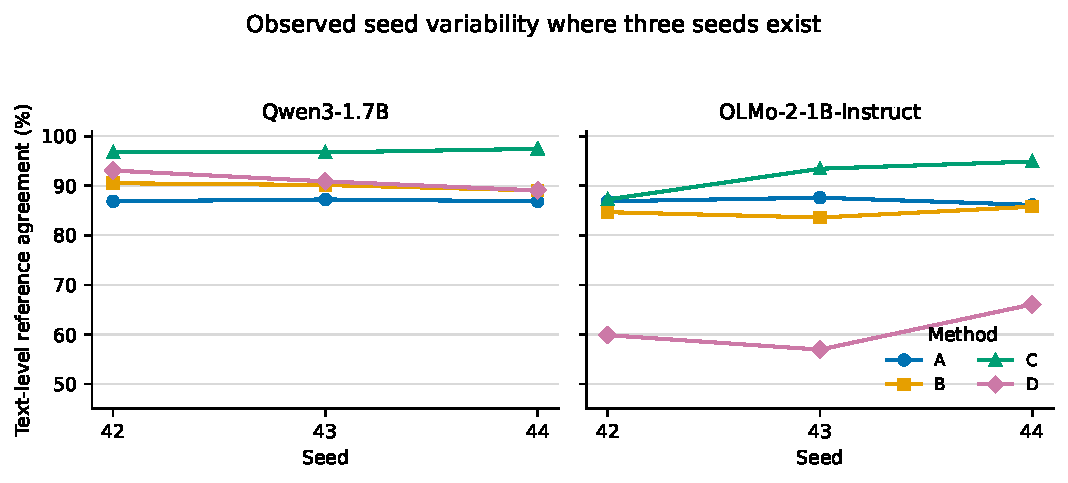
\includegraphics[width=\textwidth]{figures/text_level_seed_variability.pdf}
  \caption{Observed text-level chart-reference agreement across seeds 42--44 for the two profiles with three-seed coverage. Lines aid reading across seeds; they are not confidence intervals. The 8B and 27B profiles are omitted because only seed 42 exists. Source: \texttt{tables/format\_tolerant\_chart\_accuracy.csv}.}
  \label{fig:text-level-seed-variability}
\end{figure}


Three-seed coverage exists only for Qwen3-1.7B and OLMo-2-1B. Table 7.8 shows the spread on text-level chart agreement, which is the outcome least contaminated by the format and truncation artifacts.

\begingroup\footnotesize\setlength{\tabcolsep}{3pt}\sloppy
\begin{longtable}[]{@{}llrrrrr@{}}
\caption{Text-level chart agreement across seeds, in percent. Values are shown individually; sd is the sample standard deviation over the three seeds and is descriptive only.}\tabularnewline
\toprule\noalign{}
Model & Method & Seed 42 & Seed 43 & Seed 44 & Mean & sd \\
\midrule\noalign{}
\endfirsthead
\toprule\noalign{}
Model & Method & Seed 42 & Seed 43 & Seed 44 & Mean & sd \\
\midrule\noalign{}
\endhead
\bottomrule\noalign{}
\endlastfoot
Qwen3-1.7B & A & 86.86 & 87.23 & 86.86 & 86.98 & 0.21 \\
Qwen3-1.7B & B & 90.51 & 90.15 & 89.05 & 89.90 & 0.76 \\
Qwen3-1.7B & C & 96.72 & 96.72 & 97.45 & 96.96 & 0.42 \\
Qwen3-1.7B & D & 93.07 & 90.88 & 89.05 & 91.00 & 2.01 \\
OLMo-2-1B & A & 86.86 & 87.59 & 86.13 & 86.86 & 0.73 \\
OLMo-2-1B & B & 84.67 & 83.58 & 85.77 & 84.67 & 1.10 \\
OLMo-2-1B & C & 87.23 & 93.43 & 94.89 & 91.85 & 4.07 \\
OLMo-2-1B & D & 59.85 & 56.93 & 66.06 & 60.95 & 4.66 \\
\end{longtable}
\endgroup

The seed spread is small for the untrained conditions --- standard deviations of 0.2--1.1 pp for A and B in both families --- which is expected, since only generation sampling varies. It is larger for the trained conditions, where the training trajectory also varies: 0.4 pp for Qwen3-1.7B C but 4.1 pp for OLMo C and 4.7 pp for OLMo D. Reporting three seeds is therefore not a formality; the trained conditions in the weaker family vary by several percentage points between otherwise identical runs, which is consistent with published observations that random seeds produce measurable variation in fine-tuned language models at both aggregate and per-item level \cite{bui2025seeds}.

Two cautions apply to Table 7.8. First, the three Qwen3-1.7B seeds are not three draws from one procedure: seed 42 was trained under a different code state, a different per-device batch size and bf16 precision, while seeds 43 and 44 were trained under the current state on a Tesla T4 in fp16 (Table 6.4). Its lower contract compliance in Table 7.1 reflects that difference rather than seed noise. Second, no standard deviation is reported for Qwen3-8B or Qwen3.8-27B, because a single run cannot estimate one. The scale comparison in Section 7.3 rests on three-seed evidence at the small scale and single-run evidence at the two larger scales, and that asymmetry is a property of the evidence, not of the models.

\subsection{Paraphrase robustness}

Table 7.9 reports the two paraphrase quantities. Consistency is the share of items whose primary predicted chart is unchanged after the meaning-preserving rewrite; accuracy is pipeline agreement on the paraphrased briefs, and the delta compares it with pipeline agreement on the same items unperturbed.

\begin{landscape}
\begingroup\scriptsize\setlength{\tabcolsep}{3pt}\sloppy
\begin{longtable}[]{@{}
  >{\raggedright\arraybackslash}p{(\linewidth - 8\tabcolsep) * \real{0.2000}}
  >{\raggedright\arraybackslash}p{(\linewidth - 8\tabcolsep) * \real{0.2000}}
  >{\raggedright\arraybackslash}p{(\linewidth - 8\tabcolsep) * \real{0.2000}}
  >{\raggedright\arraybackslash}p{(\linewidth - 8\tabcolsep) * \real{0.2000}}
  >{\raggedright\arraybackslash}p{(\linewidth - 8\tabcolsep) * \real{0.2000}}@{}}
\caption{Behaviour under the paraphrase perturbation, in percent. Multiple values are seeds 42 / 43 / 44.}\tabularnewline
\toprule\noalign{}
\begin{minipage}[b]{\linewidth}\raggedright
Model
\end{minipage} & \begin{minipage}[b]{\linewidth}\raggedright
Method
\end{minipage} & \begin{minipage}[b]{\linewidth}\raggedright
Consistency
\end{minipage} & \begin{minipage}[b]{\linewidth}\raggedright
Paraphrase accuracy
\end{minipage} & \begin{minipage}[b]{\linewidth}\raggedright
\(\Delta\) vs original
\end{minipage} \\
\midrule\noalign{}
\endfirsthead
\toprule\noalign{}
\begin{minipage}[b]{\linewidth}\raggedright
Model
\end{minipage} & \begin{minipage}[b]{\linewidth}\raggedright
Method
\end{minipage} & \begin{minipage}[b]{\linewidth}\raggedright
Consistency
\end{minipage} & \begin{minipage}[b]{\linewidth}\raggedright
Paraphrase accuracy
\end{minipage} & \begin{minipage}[b]{\linewidth}\raggedright
\(\Delta\) vs original
\end{minipage} \\
\midrule\noalign{}
\endhead
\bottomrule\noalign{}
\endlastfoot
Qwen3-1.7B & A & 0.00 / 0.00 / 0.36 & 0.36 / 0.36 / 0.73 & \(\approx\) 0 \\
Qwen3-1.7B & B & 1.09 / 0.36 / 1.09 & 1.09 / 0.73 / 1.46 & \(\approx\) 0 \\
Qwen3-1.7B & C & 1.46 / 81.39 / 86.86 & 3.65 / 81.75 / 84.31 & +2.19 / +1.09 / \ensuremath{-}1.09 \\
Qwen3-1.7B & D & 0.00 / 97.45 / 98.54 & 0.36 / 89.78 / 87.59 & +0.36 / +0.36 / \ensuremath{-}1.46 \\
Qwen3-8B & A & 100.00 & 91.61 & 0.00 \\
Qwen3-8B & B & 100.00 & 82.12 & 0.00 \\
Qwen3-8B & C & 83.58 & 83.94 & 0.00 \\
Qwen3-8B & D & 69.34 & 58.39 & 0.00 \\
Qwen3.8-27B & A & 98.54 & 91.24 & \ensuremath{-}1.10 \\
Qwen3.8-27B & B & 96.72 & 83.94 & +0.36 \\
Qwen3.8-27B & C & 100.00 & 96.72 & 0.00 \\
Qwen3.8-27B & D & 100.00 & 97.45 & 0.00 \\
OLMo-2-1B & A & 1.82 / 2.19 / 2.92 & 6.57 / 4.38 / 6.20 & small positive \\
OLMo-2-1B & B & 9.12 / 10.95 / 9.49 & 22.99 / 25.55 / 23.36 & small negative \\
OLMo-2-1B & C & 2.55 / 2.92 / 2.92 & 2.55 / 3.28 / 3.28 & \(\approx\) 0 \\
OLMo-2-1B & D & 1.09 / 2.19 / 2.55 & 1.46 / 2.19 / 2.19 & \(\approx\) 0 \\
\end{longtable}
\endgroup
\end{landscape}

Both quantities are computed from the parsed runtime object, so a condition that fails the output contract shows near-zero consistency simply because neither prediction has a readable chart. The consistency values are informative only where the condition also satisfies the contract. Where that holds, the picture is clear and favourable: Qwen3-8B is perfectly consistent under both base-model conditions (100.00 \%), Qwen3.8-27B is 96.7--100 \% consistent in all four conditions, and the current-state Qwen3-1.7B fine-tuned conditions are 81.4--98.5 \% consistent. The weakest consistency among usable conditions is Qwen3-8B under D, at 69.34 \%.

Where the paraphrase does change the answer, the change is close to accuracy-neutral: no condition loses more than 1.5 pp of agreement, and eight of the sixteen conditions lose exactly nothing. Within the tested synonym family, the systems that produce usable output are stable, and the instability that does exist is not systematically in the direction of worse answers. This statement does not extend to paraphrase families that the perturbation set does not contain --- sentence restructuring, register changes, translations, or rewrites that touch the domain nouns.

\subsection{Behaviour on under-specified briefs}

The clarification rate --- the share of responses to an under-specified brief that ask for the missing information or signal uncertainty --- is at or near zero everywhere. It is 0.0 \% in every fine-tuned condition of every model (C and D, all seeds, all four models). Among the base-model conditions it reaches 3.65 \% at most (Qwen3-1.7B A, seed 42) and is 0.73 \% and 0.36 \% for the two Qwen3-8B conditions, 1.09 \% for both 27B conditions and 1.09--3.28 \% for OLMo.

The complementary quantity shows what the systems do instead. Qwen3-8B emits a complete valid record for 100 \% of the under-specified briefs under both base-model conditions, and the 27B model for 99.27 \%. The fine-tuned conditions of both larger models also stay high, at 78.1--100 \%.

The desirable behaviour on a brief with a removed constraint and a removed KPI is not necessarily a confident complete recommendation. The measured behaviour is that the systems almost never ask. Fine-tuning removes even the small tendency that the base models show, which is expected given that no training target in the frozen dataset is a clarification request: the adapters were never shown that this is a permitted response. Two limits apply to reading these numbers. The detector is a regular-expression heuristic over the generated text and will miss an implicit request for information. And the perturbation removes the constraints field, the last KPI and the last column, which does not always make a brief genuinely unanswerable. The finding is therefore reported as: under this perturbation and this detector, no condition demonstrates a reliable clarification behaviour.

\section{Failure modes}

Table 7.10 aggregates the per-item failure records. ``Parse failures'' counts items whose raw text did not yield a runtime object; ``no primary chart'' counts items for which the pipeline had no readable chart to score, which the top-1 metric records as incorrect.

\begin{landscape}
\begingroup\scriptsize\setlength{\tabcolsep}{3pt}\sloppy
\begin{longtable}[]{@{}
  >{\raggedright\arraybackslash}p{(\linewidth - 10\tabcolsep) * \real{0.1667}}
  >{\raggedright\arraybackslash}p{(\linewidth - 10\tabcolsep) * \real{0.1667}}
  >{\raggedright\arraybackslash}p{(\linewidth - 10\tabcolsep) * \real{0.1667}}
  >{\raggedright\arraybackslash}p{(\linewidth - 10\tabcolsep) * \real{0.1667}}
  >{\raggedright\arraybackslash}p{(\linewidth - 10\tabcolsep) * \real{0.1667}}
  >{\raggedright\arraybackslash}p{(\linewidth - 10\tabcolsep) * \real{0.1667}}@{}}
\caption{Failure counts per condition, out of 274 items.}\tabularnewline
\toprule\noalign{}
\begin{minipage}[b]{\linewidth}\raggedright
Model
\end{minipage} & \begin{minipage}[b]{\linewidth}\raggedright
Method
\end{minipage} & \begin{minipage}[b]{\linewidth}\raggedright
Seeds
\end{minipage} & \begin{minipage}[b]{\linewidth}\raggedright
Parse failures
\end{minipage} & \begin{minipage}[b]{\linewidth}\raggedright
Dominant parse error
\end{minipage} & \begin{minipage}[b]{\linewidth}\raggedright
Items with no primary chart
\end{minipage} \\
\midrule\noalign{}
\endfirsthead
\toprule\noalign{}
\begin{minipage}[b]{\linewidth}\raggedright
Model
\end{minipage} & \begin{minipage}[b]{\linewidth}\raggedright
Method
\end{minipage} & \begin{minipage}[b]{\linewidth}\raggedright
Seeds
\end{minipage} & \begin{minipage}[b]{\linewidth}\raggedright
Parse failures
\end{minipage} & \begin{minipage}[b]{\linewidth}\raggedright
Dominant parse error
\end{minipage} & \begin{minipage}[b]{\linewidth}\raggedright
Items with no primary chart
\end{minipage} \\
\midrule\noalign{}
\endhead
\bottomrule\noalign{}
\endlastfoot
Qwen3-1.7B & A & 42 / 43 / 44 & 273 / 274 / 273 & \texttt{schema\_error}: \texttt{encoding} is a string & 273 / 274 / 273 \\
Qwen3-1.7B & B & 42 / 43 / 44 & 271 / 270 / 271 & \texttt{schema\_error}: \texttt{encoding} is a string & 271 / 270 / 271 \\
Qwen3-1.7B & C & 42 / 43 / 44 & 270 / 44 / 33 & seed 42 \texttt{schema\_error}; seeds 43--44 \texttt{no\_json\_found} & 270 / 45 / 33 \\
Qwen3-1.7B & D & 42 / 43 / 44 & 274 / 4 / 0 & seed 42 \texttt{schema\_error}; seed 43 \texttt{no\_json\_found} & 274 / 4 / 0 \\
Qwen3-8B & A & 42 & 0 & --- & 0 \\
Qwen3-8B & B & 42 & 0 & --- & 0 \\
Qwen3-8B & C & 42 & 38 & \texttt{no\_json\_found} & 38 \\
Qwen3-8B & D & 42 & 71 & \texttt{no\_json\_found} & 72 \\
Qwen3.8-27B & A--D & 42 & 0 & --- & 0 \\
OLMo-2-1B & A & 42 / 43 / 44 & 202 / 198 / 200 & \texttt{no\_json\_found} & 262 / 255 / 258 \\
OLMo-2-1B & B & 42 / 43 / 44 & 169 / 157 / 168 & \texttt{no\_json\_found} & 201 / 191 / 199 \\
OLMo-2-1B & C & 42 / 43 / 44 & 266 / 266 / 266 & \texttt{no\_json\_found} & 266 \\
OLMo-2-1B & D & 42 / 43 / 44 & 271 / 267 / 265 & \texttt{no\_json\_found} & 271 / 267 / 265 \\
\end{longtable}
\endgroup
\end{landscape}

Two failure modes dominate, and they are distinguishable.

\textbf{Type error in the encoding field.} For Qwen3-1.7B under A and B, and under C and D at seed 42, the model returns a complete, well-formed JSON object in which \texttt{encoding} is a bare string --- typically the name of the x-axis column, for example \nolinkurl{"encoding":\ "payment_method_code"} --- rather than an object with named channels. The response is otherwise correct, including the chart type. The runtime contract rejects it, so the item is scored as a chart error. Zero of these responses are truncated. No other model in the study shows this failure.

\textbf{Truncation at the output budget.} For OLMo in all conditions, and for the fine-tuned Qwen3-8B and Qwen3-1.7B conditions, the failure is \texttt{no\_json\_found} and the cause is that the response never closed. Of the 191 OLMo prompt-only responses at seed 42 that failed to parse, 189 do not end with a closing brace. The stored prefixes are well-formed and often correct: an OLMo seed-43 fine-tuned response begins with a valid \texttt{context\_summary}, a correct \texttt{chart\_type}, and a fully populated encoding, and stops in the middle of the \texttt{having} array. The behaviour is consistent across the affected conditions: the model emits the long reference format faithfully and runs out of budget.

The Qwen3-8B row isolates this mechanism cleanly, because it is the one model where the same base produces zero truncations without an adapter and a substantial number with one. Fine-tuning raises truncations from 0 to 36 of 274, and adding retrieval on top raises them to 69. Retrieval consumes input budget and appears to lengthen the response; both effects push more items past the ceiling.

The mean raw response length is consistent with this account. OLMo prompt-only responses average about 2,150 characters and 27B prompt-only responses about 2,300, both against a hard ceiling of 512 generated tokens.

\section{Retrieval grounding}

Table 7.11 reports the grounding diagnostic for the sixteen RAG conditions. Claim coverage must be read first: it is the share of items that contributed at least one scorable rationale claim, and where it is low the supported-claim rate describes only a handful of claims.

\begin{landscape}
\begingroup\scriptsize\setlength{\tabcolsep}{3pt}\sloppy
\begin{longtable}[]{@{}
  >{\raggedright\arraybackslash}p{(\linewidth - 10\tabcolsep) * \real{0.1364}}
  >{\raggedright\arraybackslash}p{(\linewidth - 10\tabcolsep) * \real{0.1364}}
  >{\raggedleft\arraybackslash}p{(\linewidth - 10\tabcolsep) * \real{0.1818}}
  >{\raggedleft\arraybackslash}p{(\linewidth - 10\tabcolsep) * \real{0.1818}}
  >{\raggedleft\arraybackslash}p{(\linewidth - 10\tabcolsep) * \real{0.1818}}
  >{\raggedleft\arraybackslash}p{(\linewidth - 10\tabcolsep) * \real{0.1818}}@{}}
\caption{Lexical-proxy grounding for conditions B and D. All conditions retrieved documents for all 274 items.}\tabularnewline
\toprule\noalign{}
\begin{minipage}[b]{\linewidth}\raggedright
Model
\end{minipage} & \begin{minipage}[b]{\linewidth}\raggedright
Method
\end{minipage} & \begin{minipage}[b]{\linewidth}\raggedleft
Seed
\end{minipage} & \begin{minipage}[b]{\linewidth}\raggedleft
Claim coverage (\%)
\end{minipage} & \begin{minipage}[b]{\linewidth}\raggedleft
Scored claims
\end{minipage} & \begin{minipage}[b]{\linewidth}\raggedleft
Supported claims (\%)
\end{minipage} \\
\midrule\noalign{}
\endfirsthead
\toprule\noalign{}
\begin{minipage}[b]{\linewidth}\raggedright
Model
\end{minipage} & \begin{minipage}[b]{\linewidth}\raggedright
Method
\end{minipage} & \begin{minipage}[b]{\linewidth}\raggedleft
Seed
\end{minipage} & \begin{minipage}[b]{\linewidth}\raggedleft
Claim coverage (\%)
\end{minipage} & \begin{minipage}[b]{\linewidth}\raggedleft
Scored claims
\end{minipage} & \begin{minipage}[b]{\linewidth}\raggedleft
Supported claims (\%)
\end{minipage} \\
\midrule\noalign{}
\endhead
\bottomrule\noalign{}
\endlastfoot
Qwen3-8B & B & 42 & 100.0 & 832 & 63.33 \\
Qwen3.8-27B & B & 42 & 100.0 & 695 & 61.08 \\
Qwen3.8-27B & D & 42 & 100.0 & 330 & 48.33 \\
Qwen3-1.7B & D & 43 & 98.54 & 310 & 31.48 \\
Qwen3-1.7B & D & 44 & 100.0 & 304 & 31.20 \\
Qwen3-8B & D & 42 & 74.09 & 206 & 57.64 \\
Qwen3-1.7B & B & 42 & not recorded & 9 & 77.78 \\
Qwen3-1.7B & B & 43 & 1.46 & 13 & 64.58 \\
Qwen3-1.7B & B & 44 & 1.09 & 9 & 77.78 \\
Qwen3-1.7B & D & 42 & 0.0 & 0 & not available \\
OLMo-2-1B & B & 42 & 18.61 & 91 & 39.05 \\
OLMo-2-1B & B & 43 & 20.44 & 101 & 46.58 \\
OLMo-2-1B & B & 44 & 21.53 & 116 & 49.72 \\
OLMo-2-1B & D & 42 & 1.09 & 3 & 100.00 \\
OLMo-2-1B & D & 43 & 2.55 & 7 & 28.57 \\
OLMo-2-1B & D & 44 & 3.28 & 9 & 44.44 \\
\end{longtable}
\endgroup
\end{landscape}

Only six of the sixteen conditions have claim coverage above 70 \%, and only those six support a reading of the supported-claim rate. Among them, the two base-model conditions of the larger Qwen3 profiles are the highest, at 63.33 \% (8B) and 61.08 \% (27B) over 832 and 695 claims respectively. The fine-tuned-plus-retrieval conditions are lower: 57.64 \% at 8B, 48.33 \% at 27B and 31.2--31.5 \% at 1.7B. The remaining ten conditions have coverage between 0 \% and 21.5 \%, because their rationales could not be extracted from unparseable or truncated output; the OLMo D seed-42 value of 100 \% is computed over three claims and carries no weight.

Two limits bound every value in this table. Support is decided by content-word overlap, and lexical overlap is not entailment: a rationale can reuse the vocabulary of a retrieved passage without being justified by it, and it can be justified by a passage it does not lexically resemble. Retrieval relevance --- whether the retriever selected the \emph{right} passages --- was not measured at all, because the evaluation needs independent relevance judgements and none exist. The grounding numbers therefore describe how much retrieved vocabulary reappears in the rationales and nothing stronger.

\section{Computational cost}

Table 7.12 reports mean generation latency per item. The comparison across conditions is confounded by hardware and is reported as a descriptive cost record for the executed configuration only.

\begin{landscape}
\begingroup\scriptsize\setlength{\tabcolsep}{3pt}\sloppy
\begin{longtable}[]{@{}
  >{\raggedright\arraybackslash}p{(\linewidth - 8\tabcolsep) * \real{0.2000}}
  >{\raggedright\arraybackslash}p{(\linewidth - 8\tabcolsep) * \real{0.2000}}
  >{\raggedright\arraybackslash}p{(\linewidth - 8\tabcolsep) * \real{0.2000}}
  >{\raggedright\arraybackslash}p{(\linewidth - 8\tabcolsep) * \real{0.2000}}
  >{\raggedright\arraybackslash}p{(\linewidth - 8\tabcolsep) * \real{0.2000}}@{}}
\caption{Mean generation latency per item in seconds, with the inference device.}\tabularnewline
\toprule\noalign{}
\begin{minipage}[b]{\linewidth}\raggedright
Model
\end{minipage} & \begin{minipage}[b]{\linewidth}\raggedright
A
\end{minipage} & \begin{minipage}[b]{\linewidth}\raggedright
B
\end{minipage} & \begin{minipage}[b]{\linewidth}\raggedright
C
\end{minipage} & \begin{minipage}[b]{\linewidth}\raggedright
D
\end{minipage} \\
\midrule\noalign{}
\endfirsthead
\toprule\noalign{}
\begin{minipage}[b]{\linewidth}\raggedright
Model
\end{minipage} & \begin{minipage}[b]{\linewidth}\raggedright
A
\end{minipage} & \begin{minipage}[b]{\linewidth}\raggedright
B
\end{minipage} & \begin{minipage}[b]{\linewidth}\raggedright
C
\end{minipage} & \begin{minipage}[b]{\linewidth}\raggedright
D
\end{minipage} \\
\midrule\noalign{}
\endhead
\bottomrule\noalign{}
\endlastfoot
Qwen3-1.7B, seed 42 & 7.1 (A30) & 6.6 (A30) & 9.4 (A30) & 9.7 (A30) \\
Qwen3-1.7B, seeds 43/44 & 7.1 (A30) & 6.6--6.7 (A30) & 38.7--39.0 (L4) & 57.2--59.1 (T4) \\
Qwen3-8B, seed 42 & 33.0 (GB10) & 34.4 (GB10) & 22.5 (GB10) & 23.1 (GB10) \\
Qwen3.8-27B, seed 42 & 30.9 (H100 NVL) & 29.4 (H100 NVL) & 76.2 (GB10) & 81.3 (GB10) \\
OLMo-2-1B, seed 42 & 10.1 (GB10) & 10.0 (GB10) & 13.6 (H100 NVL) & 13.8 (H100 NVL) \\
\end{longtable}
\endgroup
\end{landscape}

Where the device is held constant, three regularities appear. Retrieval is close to free at generation time: B is within 1.4 s of A in every same-device pair. Loading a 4-bit quantized base model with an adapter is more expensive than running the base model in its normal precision at 1.7B, where C is 2.3 s slower than A on the same A30. And D is consistently a little slower than C, by 0.3--5.1 s.

The Qwen3-8B row is the only complete four-condition comparison on a single device, and it runs against that pattern: the fine-tuned conditions are about 11 s \emph{faster} per item than the base-model conditions. This is consistent with the response-length evidence in Section 7.2.5 --- the base-model conditions emit alternatives on all 274 items while the fine-tuned conditions emit none, so they have less to generate --- but the runs were not instrumented to measure generated token counts directly, so the explanation is not established by the artifacts.

The values across devices are not comparable. The 57--59 s per item for Qwen3-1.7B D at seeds 43/44 reflects a Tesla T4, not a property of method D; the same method on an A30 at seed 42 takes 9.7 s.

The total resource footprint of the reported experiment was approximately 162 GPU-hours of inference across the thirty-two runs and 23 GPU-hours of adapter training across the eight adapters, on five different GPU types. Training one adapter took 0.54 h for OLMo-2-1B on an H100 NVL, 1.0--3.4 h for Qwen3-1.7B depending on device, 4.9 h for Qwen3-8B and 8.8 h for Qwen3.8-27B.

\section{Human evaluation (RQ2 and RQ3)}

The final analysis excludes all test accounts and earlier rubric versions. Fifteen participants consented to the open bilingual study. Ten completed all eight assigned pages, one partial session contributed one page, and four registered participants submitted none, yielding 81 pages for 32 outputs. Each output received two to four pages. The intended three-page coverage was therefore not reached for every output, and 11 of 486 possible dimension judgements are missing. The analysis retains these missing values rather than coding them as neutral scores.

\begin{table}[htbp]
\centering
\small
\setlength{\tabcolsep}{4.2pt}
\caption{Human ratings by method, averaged within each brief and then equally across the eight briefs. Scores range from 1 (low) to 5 (high). The last column reports ordinal Krippendorff's $\alpha$ across the 32 multiply rated outputs.}
\label{tab:human-evaluation-results}
\begin{tabular}{lrrrrr}
\toprule
Dimension & A & B & C & D & $\alpha$ \\
\midrule
Chart appropriateness & 4.38 & \textbf{4.48} & 4.02 & 3.92 & 0.066 \\
Layout quality & \textbf{4.40} & 4.33 & 3.90 & 3.98 & 0.045 \\
Styling and accessibility & 4.10 & \textbf{4.33} & 4.25 & 4.21 & 0.579 \\
Interaction design & \textbf{4.58} & 4.54 & 4.13 & 4.38 & 0.062 \\
Rationale quality & 4.29 & \textbf{4.52} & 3.76 & 4.13 & 0.209 \\
Overall usefulness & 4.21 & \textbf{4.52} & 4.05 & 4.04 & 0.167 \\
\bottomrule
\end{tabular}
\end{table}

All method--dimension means lie between 3.76 and 4.58. Retrieval-only (B) has the highest equal-brief mean for chart appropriateness, styling and accessibility, rationale quality, and overall usefulness. Prompt-only (A) is slightly higher for layout quality and interaction design. The largest descriptive B--A difference is +0.31 points for overall usefulness; the layout and interaction differences favouring A are only 0.06 and 0.04 points. The fine-tuned conditions do not exceed B on any dimension. Relative to C, adding retrieval in D is associated with higher interaction (+0.25) and rationale (+0.36) scores, while overall usefulness is essentially unchanged (+0.01 for C over D).

Agreement is the principal qualification. Ordinal $\alpha$ is 0.579 for styling and accessibility but ranges from 0.045 to 0.209 for the other five dimensions. Thus, raters often disagree about the same output, especially on layout, interaction, and chart appropriateness. Together with convenience recruitment, eight briefs, shared raters, and incomplete three-page coverage, this rules out a confirmatory ranking of the four methods. The human data support a bounded descriptive conclusion: participants generally rated all four systems positively, retrieval-only obtained the strongest average profile in this sample, and the automatic reference-agreement penalty for retrieval does not translate into a corresponding decline in perceived usefulness.

Two planned automatic quantities remain outside the executed analysis. Independent chart effectiveness was not computed because its set-valued scorer is not implemented; automatic chart results are therefore agreement with the project's reference. Retrieval relevance metrics such as Recall@3, MRR@3, and nDCG@3 were also not computed because no independent relevance judgements exist.
